\section{Introduction}

Motion planning is a fundamental problem in robotics that involves computing a feasible and efficient trajectory for a robot to move from an initial configuration to a goal configuration while satisfying various constraints\cite{lavalle2006planning}.
%
The problem becomes particularly challenging in high dimensional systems, which are generally known to be PSPACE-hard\cite{reif1979complexity}.

Classical approaches to motion planning rely heavily on sampling-based planners, such as Rapidly-exploring Random Trees (RRT)\cite{lavalle2001randomized} and Probabilistic Roadmaps (PRM)\cite{kavraki1996probabilistic}, due to their ability to efficiently explore high-dimensional spaces.
%
These planners have been widely adopted because they can handle complex environments without requiring an explicit representation of the free space.
%
However, when additional constraints such as kinodynamic feasibility, obstacle avoidance, or motion continuity are introduced, these methods struggle to produce high-quality, optimal trajectories.

Recent advances in optimization-based motion planning have tackled these limitations by formulating the problem as a compact mixed-integer convex program\cite{marcucci2023motion}.
%
One such approach, the Graph of Convex Sets (GCS) framework\cite{marcucci2024shortest}, enables the encoding of collision-avoidance constraints and system dynamics within a single convex optimization formulation.
%
By leveraging convex relaxations and mixed-integer programming, GCS provides a structured way to computing globally optimal trajectories while ensuring feasibility in constrained environments.

\begin{figure}[!t]
    \centering
    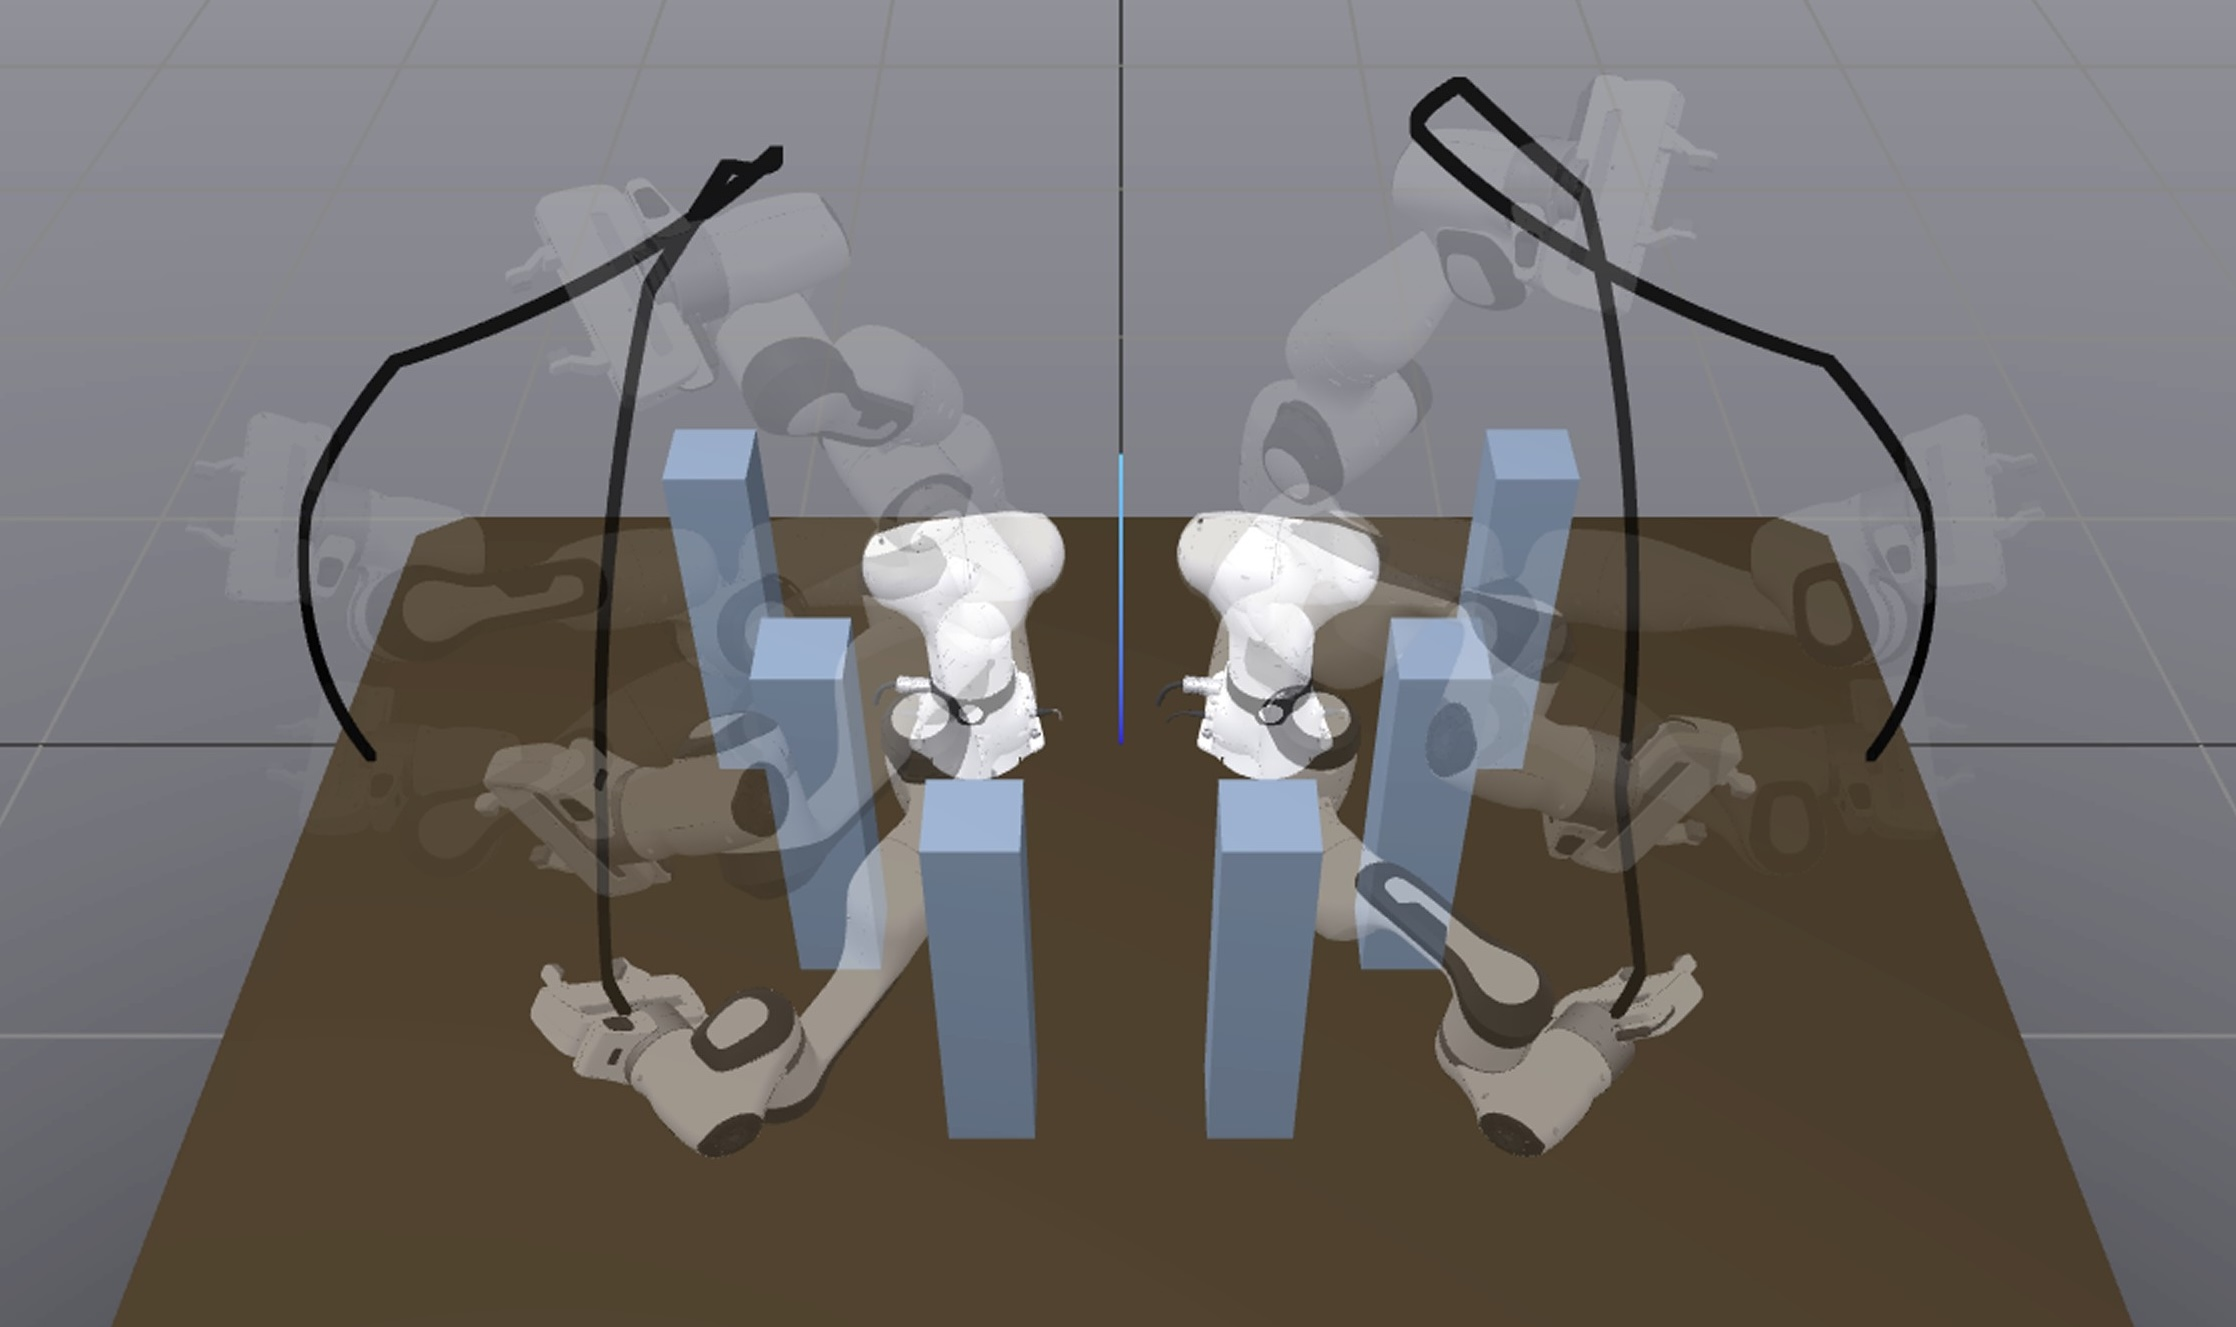
\includegraphics[width=0.99\linewidth]{figures/gcs_solution_trajectory_hd.jpg}
    \caption{A composite figure of two Franka Emika Panda robots executing a path found by our proposed convex optimization-based motion planning approach.}
    \label{fig:gcs_solution}
\end{figure}

\subsection{Contributions}
In this project, we explore the use of GCS framework for kinodynamic motion planning in dual-arm robotic manipulation (Figure~\ref{fig:gcs_solution}). Our key contributions are as follows:

\begin{itemize}
\item We formulate the problem of generating \textit{collision-free, kinodynamic motion plans} for a dual-arm manipulator as a mixed-integer convex program (MICP), following the approach in~\cite{marcucci2023motion}. However, unlike prior work, we investigate the scalability of the GCS framework in significantly higher-dimensional settings---specifically, an 18-degree-of-freedom (DOF) dual-arm system operating in a more complex, cluttered environment with narrow passages.
 
\item We conduct a comprehensive experimental study to evaluate the effectiveness of the optimization-based motion planning approach. Our experiments also include comparisons against recent sampling-based algorithms, analyzing critical performance metrics such as solution quality and computation time.
\end{itemize} 

This report is organized as follows: Section~\ref{sec:formulation} presents the problem formulation of our proposed approach. Section~\ref{sec:results} discusses and analyzes the results from our simulation studies. Finally, Section~\ref{sec:conclusion} concludes the report.